% AIIT Bulletin Template Version 17.9 2023-07-13; Equivalent Word template version: 5

\documentclass[fontsize=9pt, jafontscale=.95, twocolumn, a4paper]{jlreq}
\usepackage{authblk}
\usepackage{pbalance}
\renewcommand\Affilfont{\footnotesize\vspace{-.2mm}}
\title{PBL型教育におけるアジャイル人材育成のプラクティス:2023年度の事例}
\newcommand{\entitle}{Practice of agile development engineers in PBL: A case in 2023}
\author[1*]{中鉢 欣秀}
\author[1]{大野 寛人}
\author[1]{鈴木 真希}
\author[1]{中山 建太}
\author[1]{平田 聖}
\author[1]{Fabianmarcelo Fernandez}
\author[1]{水野 響}
\author[1]{宮原 大}
\author[1*]{\authorcr\small Yoshihide Chubachi} % add \authorcr at the beginning of the first author's latin name
\author[1]{\small Hiroto Ono}
\author[1]{\small Maki Suzuki}
\author[1]{\small Kento Nakayama}
\author[1]{\small Hijiri Hirata}
\author[1]{\small Fabianmarcelo Fernandez}
\author[1]{\small Hibiki Mizuno}
\author[1]{\small Dai Miyahara}
\affil[1]{東京都立産業技術大学院大学  Advanced Institute of Industrial Technology}
\affil[*]{Corresponding author: Yoshihide Chubachi, yc@aiit.ac.jp}
\newcommand{\abstractcontent}{Agile development is gaining recognition in the corporate world and is widely adopted for small-scale, quick-turnaround software development. However, in some cases, the actual agile development in companies is only a limited adoption of some of the methods, and the benefits of agile development are not being fully realized. There are also difficulties in introducing a full set of agile development methods, such as lack of experience among members and lack of understanding in the organization. It is highly valuable to provide a place for university education to conduct full-scale Agile development, to gain experience and knowledge, and to acquire Agile development competencies. In this paper, we describe the practices that the authors are implementing in their project-based learning in the first semester of 2023.  The significance of learning agile development at universities is that it provides an environment where students can practice an ideal and desirable development methodology in a situation where various external factors such as those that occur in practice are minimized. We need to continue to devise ways to provide a better learning environment.}
\newcommand{\keywordscontent}{agile development; project-based learning; software engineer education}
% \newcommand{\doi}{10.1000/aiit0017}
% import a package set
\usepackage{aiit}

% load settings for layouts and aesthetic tweaks.
% comment this out to speed up compile (draft quality)
\usepackage{aiit-aes}

\begin{document}
% AIIT Bulletin Template Version 17.9 2023-07-13; Equivalent Word template version: 5
\twocolumn[%
\vspace{-15mm}
\maketitle
\vspace{-8mm}
\begin{spacing}{.8}
\begin{onecolabstract}
\abstractcontent
\end{onecolabstract}
\small\textbf{Keywords\quad}\keywordscontent\\
\vspace{2mm}
\rule{\textwidth}{.1mm}
\end{spacing}
\vspace{8mm}
]
\pagestyle{aiit}


\section{はじめに}
\label{sec:org7c2856a}
企業におけるアジャイル開発の認知度は高まっており,小規模単納期型のソフトウェア開発に広く採用されてきている.しかしながら,実際に企業で行っているアジャイル開発では,手法の一部を限定的に取り入れているに過ぎず,アジャイル開発の恩恵を十分に受けられていないケースが見られる.フルセットのアジャイル開発を導入しようとしてもメンバーに経験が無い,組織の理解が得られていない等の困難さもある.

大学教育において,本格的なアジャイル開発を行い,経験や知識を得てアジャイル開発のコンピテンシーを獲得するための場を提供することの価値は高いと言える.

本論文では,2023年度前期において筆者らが実践しているプロジェクト型学習で行っているプラクティスについて述べる.

筆者らはアジャイル開発に対応できる技術者の育成を大学におけるPBL型教育で行う取り組みを実践している\cite{中鉢1608,中鉢1609,中鉢1610,中鉢1611-el,中鉢1701,中鉢1712-AIIT,中鉢1809,中鉢2009-FIT}.これらは2012年度に始まったenPiT\cite{井上14}のビジネスアプリケーション分野\cite{嵯峨17}で大学におけるスクラムの教育から得られた知見を発展させ,実施しているものである.


直近の事例として,2021年度の事例を文献\cite{中鉢2112,中鉢2109}に,2022年度の事例を文献\cite{中鉢2301,中鉢2209}で発表している.本論文はこれらに続く2023年度の事例であり,本年度前期PBL成果発表会にて学生が作成した発表資料と日本ソフトウェア科学会大会講演論文\footnote{著作権は筆者らが有する}に基づいて構成したものである.

以下,2.ではプロジェクトのメンバー構成,3.ではプロダクトの決定から開発までの流れを示し,4.で考察し,5.でまとめを行う.

\section{メンバー構成}
\label{sec:org995f5e0}

本学は社会人学生の比率が高く,情報アーキテクチャコースにおいては情報技術分野に関連する仕事の経験者が多く在学する.

2023年度は7名の学生がプロジェクトに参加している.技術者として経験を有するのはそのうち4名である.その内訳は表\ref{tab:org97f5891}に示す通り,Webのフロントエンドの技術,バックエンドの技術,及びインフラストラクチャーに関する技術である.ここでフロントエンドの技術者とは,HTML/CSS/JavaScriptを用いて主としてユーザに提供するインターフェース部分に関連する技術を備える者である.次に,バックエンドの技術者とは,Webサーバーやデータベースを用いてサーバーサイドにある主としてロジック部分に関連する技術を有する.最後に,インフラストラクチャーの技術とは,ネットワーク技術の知識を有することを示す.

本年度は,バックエンドの技術的経験を持つメンバーが比較的多かった.この内3名はテックリードとして他のメンバーを指導する役割を担うことのできる技術レベルを有する.

\begin{table}[tb]
\caption{\label{tab:org97f5891}経験のある技術}
\centering
\begin{tabular}{ll}
技術 & 人数\\
\hline
Webフロントエンド & 1名\\
Webバックエンド & 3名\\
インフラストラクチャ & 1名\\
未経験 & 2名\\
\end{tabular}
\end{table}

また,スクラムの経験については表\ref{tab:org7cb6fee}に示す.7名中5名が一定の経験を有している.

\begin{table}[tb]
\caption{\label{tab:org7cb6fee}スクラムの経験}
\centering
\begin{tabular}{ll}
技術 & 人数\\
\hline
経験あり & 1人\\
若干の経験あり & 4人\\
未経験 & 2人\\
\end{tabular}
\end{table}

技術面では3名のテックリードがいる一方,スクラムについては全体的に習熟度が低い状況である.特にフルセットのスクラムを経験したものはいなかった.

ここで,フルセットのスクラムとはプロジェクトの開始から終結まで一貫としてスクラムによる開発手法を中核として用いることを前提としたシステム開発を行うことを言う.

本年度はこのようなメンバー構成で「スクラムマスターに求められるスキルを身につける」ことを目標に,プロジェクト活動を行っている.

\section{プロダクトの決定から開発まで}
\label{sec:org464a68f}

\subsection{開発の事前準備}
\label{sec:org91b6723}

スクラムはソフトウェア開発の手法であり,プロダクトそのものをデザインする方法については言及していない.そのため,プロダクトデザインの方法は開発チームの検討に委ねられる.また,この作業は開発スプリントに入る前に実施する.チームでは次の流れで開発するプロダクトを決定した(図\ref{fig:プロダクト開発の流れ}).

\begin{enumerate}
\item 目標設定
\item 何を作るか
\item 価値は何か
\item 価値の確認
\item 役割決め
\item スプリント開始
\end{enumerate}

\begin{figure}[tb]
\centering
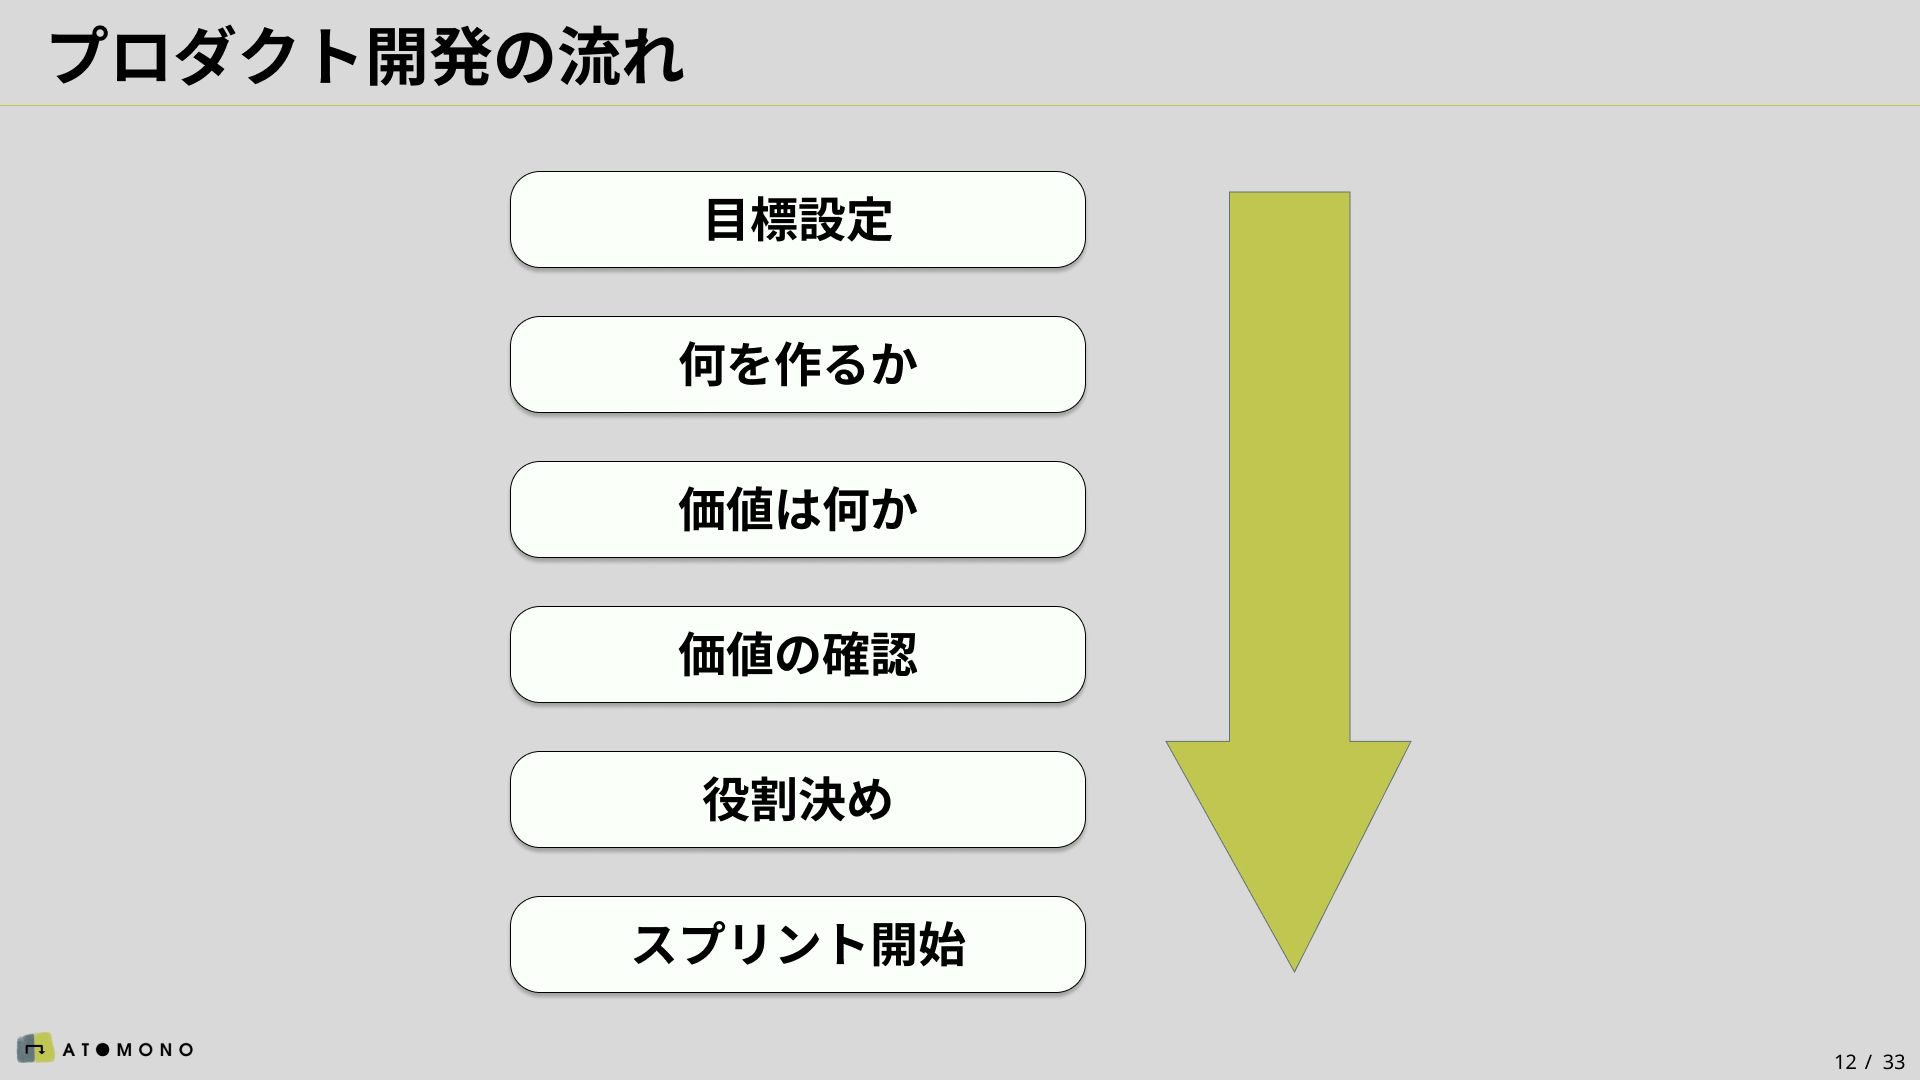
\includegraphics[width=.9\linewidth]{./images/前期発表資料_ページ_12.png}
\caption{\label{fig:プロダクト開発の流れ}プロダクト開発の流れ}
\end{figure}

以下,それぞれについて説明する.

\subsection{目標設定}
\label{sec:org3653438}

PBLは学習のメソッドであり,成果はあくまでもチームメンバーがスキルやコンピテンシーの獲得することである.その過程において,実際にソフトウェアプロダクトを開発し,課題解決を行うことで実践的な学びを深めるのがソフトウェア開発型のPBLである.

今年度のチームでは目標として「個人開発スキルの向上」と「スクラムマスターの役割の習得」の2つを掲げた.個人開発スキルについては,向上度合いを可視化するため,各技術レイヤーごとに目標を設定した.

スクラムマスターの役割に関しては,求められるスキルとして次の5つが知られている\footnote{\url{https://www.odd-e.jp/article\_009\_1/}}.

\begin{description}
\item[{ティーチング(Teaching)}] %% 文末の全角スペースは必要

知識や技術を教え与える
\item[{ファシリテーティング(Facilitating)}]

活動(チーム活動や議論等)を促進する
\item[{メンタリング(Mentoring)}]

対話を通じて人生観などに対する気づきを促す
\item[{コーチング(Coaching)}]

問題解決や目標達成のための気づきを促す
\item[{シチュエーショナリング(Situationaling)}]

状況を把握して対応する
\end{description}

メンバーはこのうち「メンタリング」を除く4つを獲得することを目標に設定し,知識の習得レベルをパラメーター化することで可視化することにした.

以上のように,学習目標を明確に定め,習得状況を可視化して学習の達成度を明確にすることで,学習の励みになり,学習成果に結びつくことが期待できる.

\subsection{何を作るか}
\label{sec:org0a7ccf8}
プロジェクトで開発するプロダクトを決定するために,アイデアソンを実施した.いくつかのアイデアが得られ,投票を行うことで何を作るかチーム内で合意を形成した.

2023年度前期は「お気に入りの化粧品が廃盤になったときに,代替品をすぐに探せるようにする」サービスをテーマとすることになった(図\ref{fig:プロダクトの概要}).お気に入りの日用品が販売されなくなった場合に代替品を探すのが大変だというメンバー共通の悩みがあったことから,ターゲットをより限定して日用品のカテゴリを「化粧品」とした.

\begin{figure}[tb]
\centering
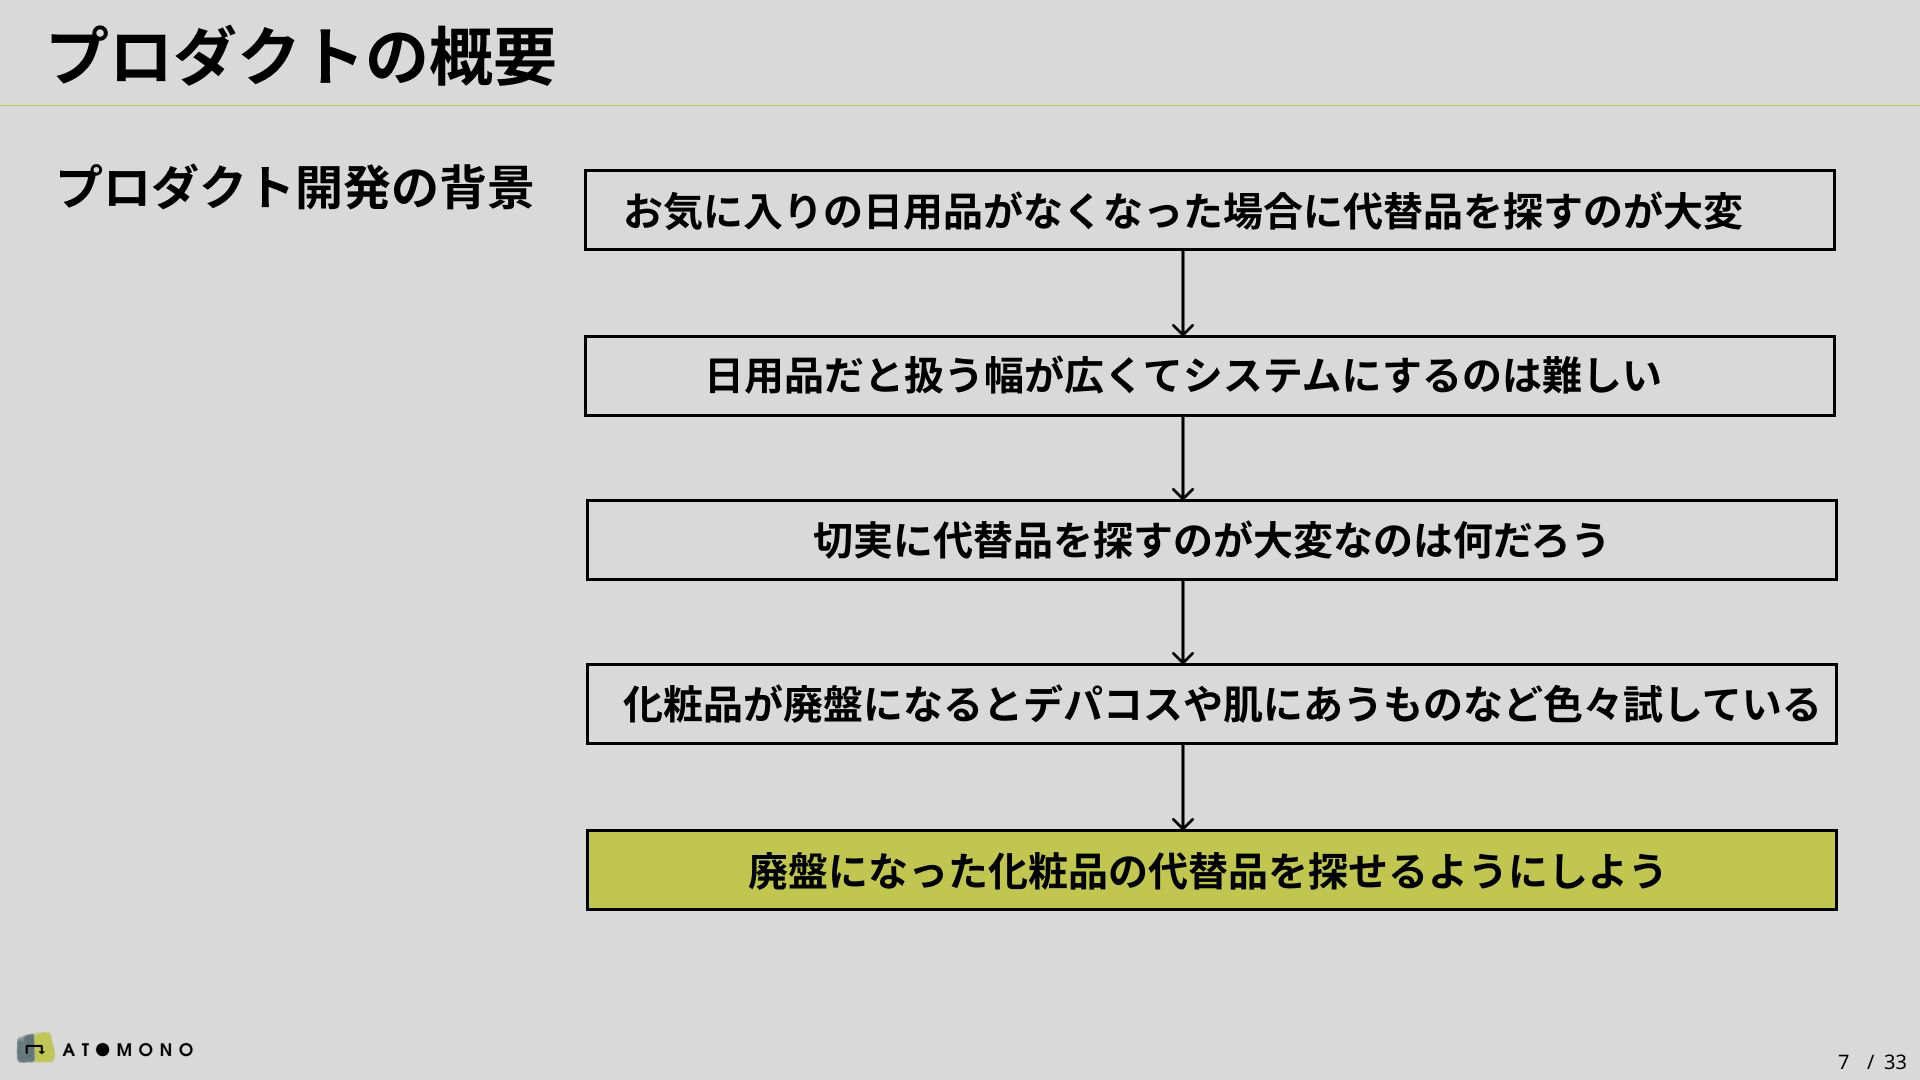
\includegraphics[width=.9\linewidth]{./images/前期発表資料_ページ_07.png}
\caption{\label{fig:プロダクトの概要}プロダクトの概要}
\end{figure}


PBLで開発するソフトウェアを決める際には,PBLの期間内に実装ができる程度の規模感や難易度が望ましい.加えて,チームメンバーが意欲を持って開発に取り組めるかが大きな鍵となる.アイデアソンとアイデアの投票という過程を経て,メンバーの合意のもとでテーマが選定された.

\subsection{価値は何か}
\label{sec:orgb96f597}
プロダクトが提供する価値を明確にすることは,完成品が備えるべき機能やサービスを決定するために重要である.「誰が」「なんのために」利用するものなのかを明確に設定しておくことが求められる.

チームでは,ペルソナとして「28歳女性」「一人暮らしの倹約家」「趣味はショッピング」といった属性を定義し,サービスを利用するユーザとして想定した.また,MVP(Minimum Viable Product)として,「化粧品の情報を調べることができる」「化粧品が廃盤になっていることを知ることができる」「代替品を探すことができる」等とした.

これらにより,プロダクトの提供する価値についての定義がなされ,開発すべきソフトウェアの姿が明確となった.

\subsection{価値の確認}
\label{sec:orgfc0adef}

\begin{figure*}[tb]
\centering
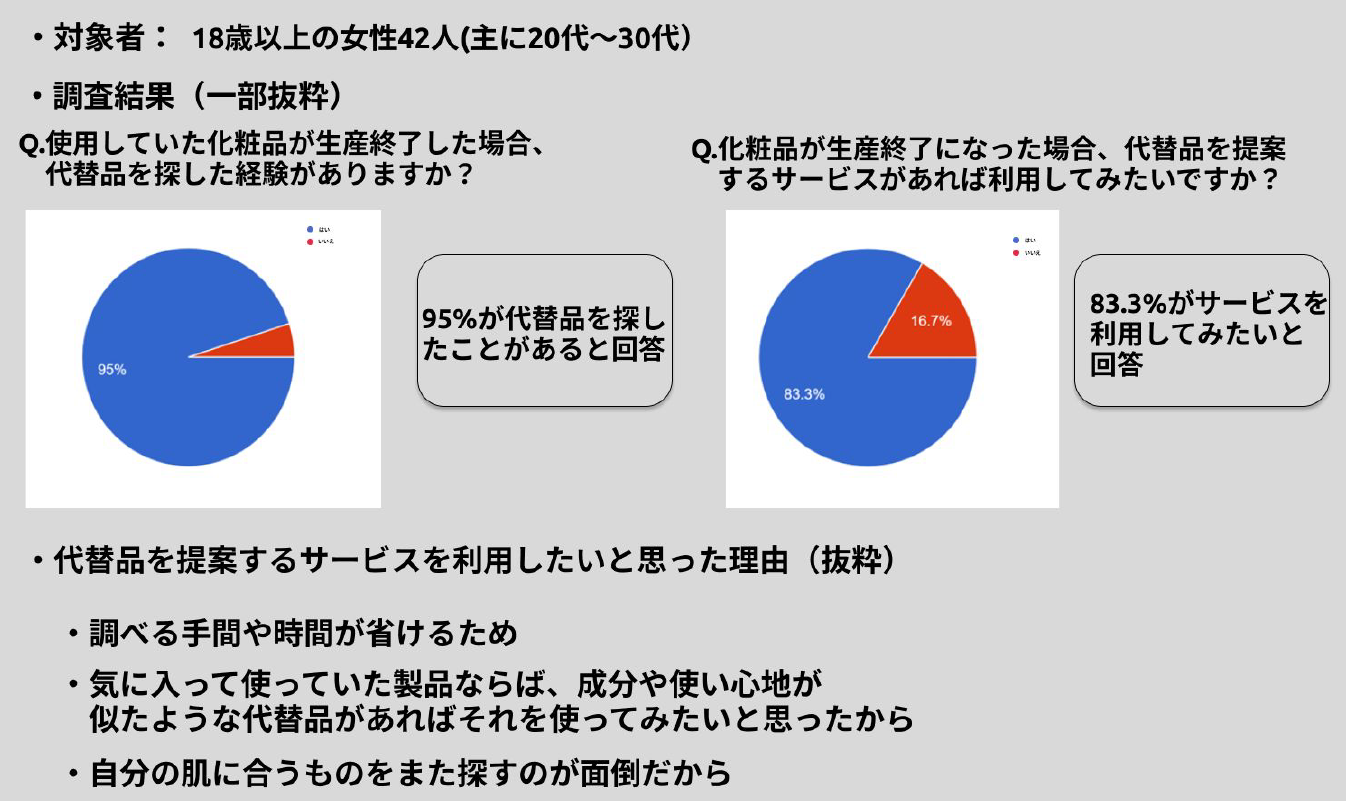
\includegraphics[width=.9\linewidth]{./images/marketing.png}
\caption{\label{fig:orgad24bd8}市場調査の結果}
\end{figure*}

チームで決定したプロダクトの価値が利用者に受け入れられるか確認するために,アンケートによる市場調査を行った.図\ref{fig:orgad24bd8}にその結果を示す.18歳以上の女性42人に調査したところ83.3\%がこのサービスを利用してみたいと回答した.

加えて,取り扱う商品のカテゴリが近い企業1社の協力を得て,製品の価値に関するインタビューを行い,意見交換をすることができた.

\subsection{役割決め}
\label{sec:org32a315d}

開発するプロダクトの概要を決めるとともに,スクラムで開発を行うための役割分担を行った.本年度の開発ではプロダクトオーナーは固定することとした.一方,学習目標に設定した通り,メンバーはスクラムマスターの役割を経験して,必要な能力の獲得を目指しているため,スクラムマスターは毎月ローテーションすることとした.

\subsection{スプリントの進め方}
\label{sec:orgea59ba2}

スプリントの進め方は昨年度の方式を踏襲することとした.スプリントの期間は一週間とし,教員との週次ミーティングを起点とし,一連のスクラムイベントを実施する.詳細については文献\cite{中鉢2209}で述べている.

チームではKPT方式で振り返りを行い,発生した課題と改善策について話し合った.課題としては次のものがあがり,それぞれについて対策を講じた.

\begin{description} %% 文末の全角スペースは必要
\item[{会議が長時間になる}]

各アジェンダに対して時間配分を設定し,ファシリテーションにより時間を管理する
\item[{スケジュールが遅延する}]

プロダクトオーナー,スクラムマスターで定期的にスケジュールを見直す
\item[{KPTのTRYの形骸化}]

前週のTRYを翌週に確認し,各スプリントのTRYを集約する
\item[{メンバー間のスキル差}]

テックリードによるSlackでのQAやサポート
\end{description}

その他,チーム内のコミュニケーションを円滑にするための工夫などが課題としてあがり,メンバーが自分たちで考えて克服した.

\section{考察}
\label{sec:org365d5f3}
このプロジェクトでは立ち上げから終結までアジャイル型の開発プロセスを経験することが大きなテーマである.ITエンジニアは日常の業務で課せられた技術については深く習得する機会がある一方,担当する業務の範囲を超え,プロダクトの企画から実装,運用までの一通りの流れを経験する機会には恵まれないことが多い.

大学におけるPBL型教育において,これら一連の開発工程をすべて経験できることはエンジニアにとっては有益な機会であると捉えている.本年度のプロジェクトでは,アイデアソン,ペルソナの設定,MVPの定義,更には市場調査などの開発エンジニアが普段経験できない事柄を実施することができた.企業へのインタビューについては,社会人「学生」としての立場を有効に活用することで企業の協力が得やすかった側面もある.

近年,企業の実際のプロジェクトでもスクラムの導入は進んできているが,フルセットのスクラムを実施することが難しいことから,スクラムを中途半端に導入していること表す「なんちゃってスクラム」という言葉も耳にする.基本に忠実に,できるだけフルセットのプロセスを経験することで,スクラムマスターとしての能力向上に寄与できる機会を提供できる.

\section{関連研究}
高等教育におけるPBLチームのプロジェクト及びチーム管理について分析した文献\cite{Fernandes2021}によれば,チーム開発を円滑に進めるためにスクラムマスターとプロダクトオーナーの役割が重要であることを学生が認識したことを指摘している.本来,スクラムマスターは,スクラムについて深く理解し,チームが望ましいスクラムの状態を保っていることを判断できるだけの知識や能力を有していることを想定している.しかしながら,初学者はそのような知識を持ち合わせていないため,プロジェクトの経験を積みながら段階的に学習する過程が必要となる.本プロジェクトでは,プロジェクトメンバーが月毎に入れ替わりでスクラムマスターを経験する.このような仕組みは実務では導入しづらいものと考えられ,PBL型の教育だからこそ実現できるものである.

López\cite{Lopez2019}らは生涯学習における不確実性への対処,適応性,創造性,対話,敬意,思いやりなどの能力を伝達するための教育としてアジャイル開発の基本的な考え方との親和性が高いと延べ,持続可能な開発のための教育(ESD)の観点からの考察を行っている.アジャイル開発はソフトウェア開発手法ではあるものの,根本的にはチームによる協調作業を円滑にする方法論である.本学のような社会人学生が多い教育の場において,様々な背景を持つチームメンバーがコラボレーションするための土台として機能することは本論文で述べた事例においても確認できる.

ソフトウェア開発PBLにおいてスクラムを実施する際,タスクの種類や量が偏りがちになることからチケット駆動を導入し,プロジェクトを定量的に評価する方法が提案されている\cite{井垣15}.本論文で述べた事例ではこのようなチケット駆動を用いた定量的な評価は実施していない.しかしながら,チームが用いているプロジェクト管理ツール等の情報を利用してより定量的な分析に基づきチームの状況を判断するための材料を得ることは可能であるため,今後の研究課題としたい.

\section{まとめ}
\label{sec:org8b3740d}
本学の情報アーキテクチャコースにおける7つのPBLのうち,ソフトウェア開発をテーマとするプロジェクトの殆どがアジャイル開発やリーン開発を採用するようになった.また,従来はアジャイル開発を経験したことのない学生が大多数であったが,近年は何らかの形でアジャイル開発を経験しており,更に深く学びたいと希望する学生の方が多くなってきている.

その背景には,一部の先駆的な企業以外では,アジャイル開発を部分的にしか導入できていないという現実がある.あるいは,プロダクトのデザインから開発までの一連の流れを全て経験することができていないという状況もある.

このような中において,大学でアジャイル開発を学習する意義は,実務で発生するような様々な外的要因が極力少ない状況で,理想的な望ましい開発方法論を学生が実践できる環境を用意できることにある.今後とも,より良い学習環境を提供するために引き続き工夫をしていく必要がある.

% \bibliography{./bibliography/references}
\printbibliography

\end{document}


%%%%%%%%%%%%%%%%%%%%%%%%%%%%%%%%%%%%%%%%%%%%%%%%%%%%%%%%%%%%%%

\section{TODO:はじめに}

本稿では、2023年度に更新された東京都立産業技術大学院大学研究紀要の新しい執筆用のTeXテンプレートファイル\cite{Matsui2023-lk}について記す。編集委員は提出された原稿をチェックはするが、体裁を整えることはしないので、無編集で公開しても問題ない品質に仕上げるための方法を説明する。

原稿は、日本語もしくは英語による完全版下 (camera ready) 原稿とする。製版後の校正は原則として不可能であるため、誤字や脱字がないよう、特に念を入れて仕上げる。刷り上がりは6ページ以上が望ましい。余白や段組、使用するフォントやフォントサイズを変更せず、そうしなければ論文としての体裁が整わないのでない限りこのテンプレートファイルに用意されたスタイルのまま仕上げる。

\subsection*{環境}

コンパイラにはLuaLaTeXを使用し、\verb|main.tex|をコンパイルする。\verb|aiit.sty|は記述に必須のパッケージが入っているので常に\mintinline{latex}{\usepackage{aiit}}としてインポートするべきだが、\verb|aiit-aes.sty|はレイアウトやヘッダー・フッターのスタイリングなどに関する設定が入っているため、下書きの段階では\mintinline{latex}{\usepackage{aiit-aes}}の行はコメントアウトしておいてもよい(コンパイルが少し早くなる)。TeX Liveのバージョンは2022を想定している。クラウド上でTeX文書を編集・生成できるサービスOverleaf\cite{Matsui2023-lk}での利用を想定しているが、自らの責任においてCloud LaTeXやローカル環境で使用してもよい。後述するmintedパッケージはPygmentsを使用するため、Overleaf以外の環境で本テンプレートを使用する場合はPygmentsをインストールするか、mintedに関連する記述を削除し、デフォルトの\verb|\verb|や\verb|\verbatim|を用いる。

\section{表題、著者名、概要}

\subsection*{表題}

表題は\mintinline{latex}{\title{}}の中に、副題は題のあとに: に続けて表記する。表題の英訳は\verb|main.tex|内の\mintinline{latex}{\newcommand{\entitle}{Title of the paper: subtitle here}}にSentence caseで記述する。

\subsection*{著者名}

著者名はauthblkパッケージを用いて以下の要領で記述する。ローマ字表記には原則としてパスポート表記と同様のヘボン式を用いる(例:ItouでもItōでもなくIto、SenoでもSenōでもなくSenoo)。所属が複数ある場合は番号を半角コンマで区切って表記し、番号の間には半角スペースを入れない。責任著者の連絡先は番号付きの所属と同様に記述し、記号には番号ではなく*を用いる。“Corresponding author: [First name] [Family name], [メールアドレス]”として表記する。コロンのあとや半角カッコのまえに半角スペースを挿入すること。原則として責任著者が退職・修了後も連絡がとれるように少なくとも今後10年間は受信できる予定のメールアドレスを記述する。

\begin{minted}{latex}
\author[`所属を表す肩付き文字`]{`著者の氏` `名`}
\author[`所属を表す肩付き文字`]{\authorcr \small `著者の氏ローマ字表記` `筆頭著者の名ローマ字表記`}

\affil[`肩付き文字`]{\footnotesize `所属の和文表記`  `所属の欧文表記`}
\affil[*]{\footnotesize Corresponding author: `責任著者の氏ローマ字表記` `責任著者の名ローマ字表記`, `責任著者のメールアドレス`}
\end{minted}

\subsection*{概要・キーワード}

論文の概要文は\mintinline{latex}{\newcommand{\abstractcontent}{abstract here}}に英語で250語以下で記述する。英語は米国英語でも英国英語でも構わないが、どちらかに統一する。イタリック体以外の太字・下線・複雑な数式・参考文献の引用は不可。著者全員の責任において破綻のない英文を作成すること。

キーワードは概要の直後の\mintinline{latex}{\newcommand{\keywordscontent}{keywords here}}に記述する。キーワードはlower caseで記述(Keyword; Keywordではなくkeyword; keyword)し、セミコロン(;)で区切る。

% DOIは各論文に割り振られたものを\mintinline{latex}{\newcommand{\doi}{10.1000/aiit0017}}の行に記述する。

\section{本文の編集}

日本語中のかっこは全角かっこ()を、英語中のかっこは半角スペースに囲まれた半角かっこ () を用いる。単位と数値のあいだには半角スペースを追加する。ルビは\ltjruby{東京|都立|産業|技術|大学院|大学|研究|紀要}{とうきょう|とりつ|さんぎょう|ぎじゅつ|だいがくいん|だいがく|けんきゅう|きよう}のようにふることができる。

\subsection*{見出し}

研究紀要は大学に所属する教員や学生が研究内容を対外的に簡潔に発信するためにある。そのため、複数のトピックを扱う学位論文のような媒体でしばしば見られる1.1.1.1のような細分化された見出しは不要である。最も大きい見出しである章には\mintinline{latex}{\section{title here}}を、節には番号をふらない\mintinline{latex}{\subsection*{title here}}を適用する。内容が簡潔であれば節に細分化せず、章のみで記述しても問題はない。

\subsection*{句読点}

和文の句読点には、全角ピリオド(.)と全角コンマ(,)の組み合わせ、もしくは「、。」の組み合わせを用いる。どちらを利用してもよいが、どちらかに統一し、スタイルが混在してはならない。また、英文の句読点には半角ピリオドと半角スペース(. )、半角コンマと半角スペース(, )を用いること。

\section{図表、コード、数式}

\subsection*{図}

図は小さいものであれば図\ref{figure:figureExample}のように1カラムいっぱいの幅(86 mm)で出力し、大きいものは図\ref{figure:figureExampleLarge}のように余白を除いた紙面いっぱいの幅(186 mm)で出力する。\verb|\label|は\verb|\caption|の直後に記述する。

図の品質は印刷に十分耐えうるものでなければならない。刷り上がり時の文字が小さすぎないよう十二分に配慮し、線の太さにも注意する。また、図表の余白にも注意する。図の具体的な描画方法については規定しないが、軸や目盛り線の太さは0.15 mmを推奨し、パネルキャプションや凡例、軸名、数値ラベルなどのフォントサイズは6 ptを推奨する。

\begin{figure}
  \centering
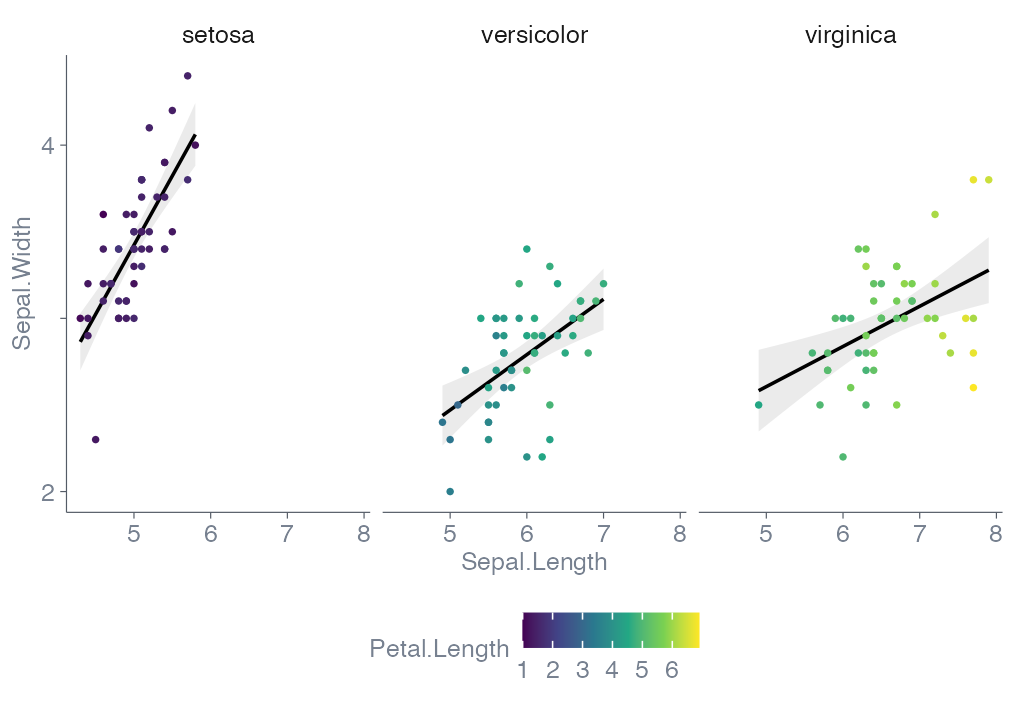
\includegraphics[width=89mm]{p_plot}
    \caption{1カラムの横幅89 mmサイズの図の例。}
    \label{figure:figureExample}
\end{figure}
\begin{figure*}[hbt!]
  \centering
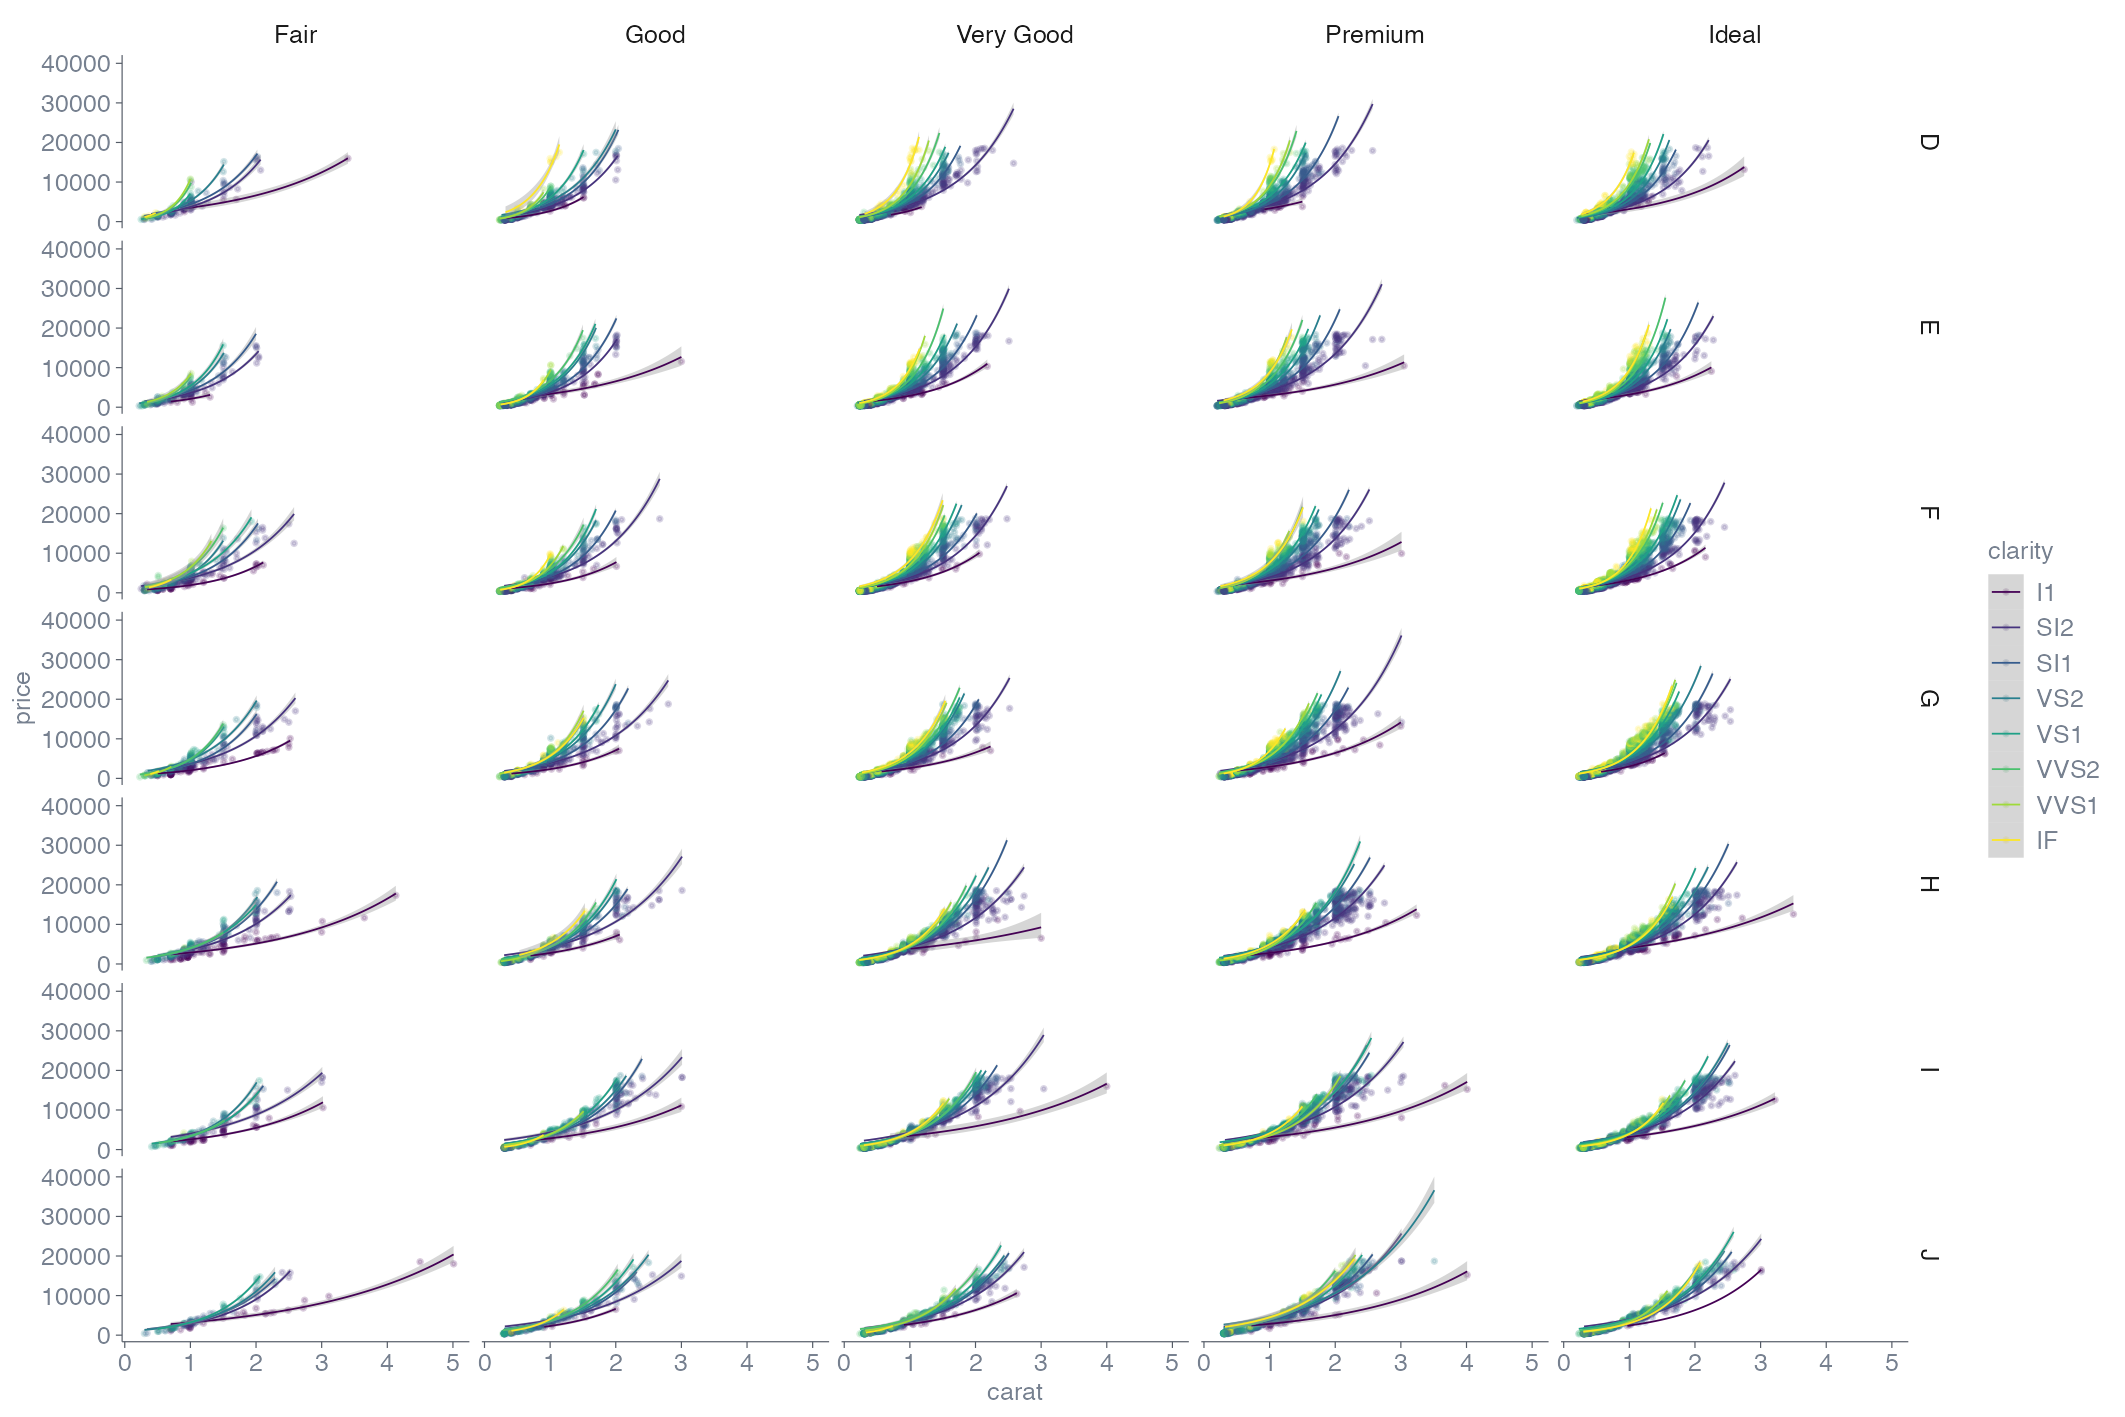
\includegraphics[width=\textwidth]{p_plot2}
    \caption{1カラムの横幅186 mmサイズの図の例。}
    \label{figure:figureExampleLarge}
\end{figure*}

\subsection*{表}

tabular環境を用いた標準的な表の例を表\ref{table:tableExample}に掲載する。

\begin{table}[hbt!]
 \caption{表の例}
 \label{table:tableExample}
 \centering
    \begin{tabular}{lllll}
        \toprule
        \multirow{2}{*}{Models} & \multicolumn{3}{c}{Metric 1} & Metric 2\\
        \cmidrule{2-4} \cmidrule{5-5} \\
        {} & precision & recall & F-score  & R@10 \\
        \midrule
        model 1 & 0.67  & 0.8 & 0.729  & 0.75 \\
        model 2 & 0.8 & 0.9 & 0.847 & 0.85 \\
        \bottomrule
    \end{tabular}
\end{table}

\subsection*{コードブロックとインラインコード}

コードブロックを挿入するには\verb|\verbatim|を用いるか、mintedパッケージを利用する。前述したように後者の利用にはPygmentsのインストールが必須である(Overleafには事前にインストールされているため不要)。以下にその例を示す。スクリプトの内容は、前述の図中の文字や軸の太さの節で推奨した設定を、R\cite{R_Core_Team2022-ar}の{tidyverse}\cite{Wickham2019-ex}ライブラリを用いてggplot2のテーマとして規定したものである。言語を設定するには\mintinline{latex}{\begin{minted}{language}}の\verb|language|部分を変更する。

\begin{minted}{r}
library(tidyverse)
theme_aiit <-
  theme_minimal(6, base_family = "Helvetica") +
  theme(
    line = element_line(linewidth = .1/.75, colour = "#545B66"),
    text = element_text(size = 6, colour = "#778190"),
    title = element_text(size = 6, colour = "#778190"),
    panel.grid = element_blank(),
    axis.line = element_line(),
    axis.text = element_text(size = 6, colour = "#778190"),
    axis.ticks = element_line(),
    plot.background = element_rect(fill = "white", colour = NA),
    strip.text = element_text(size = 6),
    strip.switch.pad.grid = unit(2, "mm"),
    strip.placement = "outside",
    legend.text = element_text(size = 6),
    legend.key.size = unit(3, units = "mm"),
    plot.tag = element_text(
      size = 10,
      family = "Helvetica",
      face = "bold"
    )
  )
\end{minted}
このテーマで例に示した図\ref{figure:figureExample}をプロットするには、以下のようにする。
\begin{minted}{r}
iris |>
  ggplot(
    aes(
      x = Sepal.Length,
      y = Sepal.Width,
      colour = Petal.Length,
      group = Species)
  ) +
  geom_smooth(
    method = "lm",
    size = .3/.75,
    colour = "black",
    fill = "grey80"
  ) +
  geom_point(size = .15/.75) +
  scale_x_continuous(breaks = 5:8) +
  scale_y_continuous(breaks = 2:4, labels = c(2, "", 4)) +
  scale_colour_viridis_c() +
  facet_wrap(vars(Species)) +
  theme_aiit +
  theme(legend.position = "bottom")
ggsave("./output/p_plot.png", width = 86, height = 60, unit ="mm", dpi = 600)
\end{minted}

同様に図\ref{figure:figureExampleLarge}をプロットするスクリプトは以下の通り。

\begin{minted}{r}
diamonds |>
  ggplot(aes(carat, price, colour  = clarity)) +
  geom_point(size = .15/.75, alpha = .2) +
  geom_smooth(
    method = "glm",
    method.args = list(family = gaussian(link = "log")),
    size = .2
  ) +
  facet_grid(cols = vars(cut), rows = vars(color)) +
  scale_colour_viridis_d() +
  theme_aiit
ggsave("./output/p_plot2.png", width = 180, height = 120, unit = "mm", dpi = 600)
\end{minted}

変数を本文中で言及する場合はたとえば\verb|\verb|を用いると\verb|date|となり、シンタックスハイライトを使いたい場合は\verb|\mintinline{language}{content}|を用いると\mintinline{r}{function(x) {x + 1}}となる。

\subsection*{数式}

数式の例を以下に示す。数式を参照するには\verb|\label|と\verb|\eqref|を使い、\eqref{eq:example}式のようにする。

\begin{equation}
\left( \int_0^\infty \frac{\sin x}{\sqrt{x}} dx \right)^2=
\sum_{k=0}^\infty \frac{(2k)!}{2^{2k}(k!)^2} \frac{1}{2k+1}=
\prod_{k=1}^\infty \frac{4k^2}{4k^2 -1}= \frac{\pi}{2} \label{eq:example}
\end{equation}

\begin{equation}
  c = 299{,}792{,}458 \, \mathrm{m/s}
\end{equation}

\begin{equation}
  A = \begin{pmatrix}
        a_{11} & \ldots & a_{1n} \\
        \vdots & \ddots & \vdots \\
        a_{m1} & \ldots & a_{mn}
      \end{pmatrix}
\end{equation}

\section{参考文献の引用}

本テンプレートの引用にはcitation-style-languageパッケージを用いているが、著者の責任においてbibtexやbiblatexなどを用いてもよい。本テンプレートファイルでは一例として、PaperPileを利用して参考文献を管理し、PaperPileのWorkflows and Integrations機能からOverleaf Integrationを選択したのち、発行されたURLを利用してオンラインのファイルを\verb|bibliography.bib|として接続している。デフォルトの設定のままでは\"{u}のような特殊文字の表示は、\mintinline{latex}{\"{u}}のように書くとコンパイルが失敗する(コンパイルがいつまで経っても終わらない)ので、\mintinline{text}{author = "Müller-Brockmann, Josef"}のように直接UTF-8で記述する必要がある(この問題はTeX Live 2023では解決済みのようなので、近日中に解決するかもしれない)。PaperPileでは設定でこの問題を回避できる。Settings\textgreater BibTeX\textgreater Escape UTF-8 charactersのチェックを外している。同様に、Include identifiers (doi, pmid)とInclude URLsにチェックを入れ、Include abstractとInclude keywordsのチェックを外した。Zoteroの場合は、\href{https://github.com/zepinglee/citeproc-lua/issues/24}{citation-style-languageの開発者が推奨する}ように\href{https://retorque.re/zotero-better-bibtex/}{Better BibTeX}を使う方法がある(未検証)。

引用方式はPLOS形式を用いる。引用方式は\mintinline{latex}{\cslsetup{style=plos}}で指定済みである。\verb|style=plos|はフォルダに格納済みの\verb|plos.csl|に紐付けられているため、このファイルを削除したりしないこと。PLOS形式はヴァンクーヴァー形式のヴァリアントで、本文中での引用を(1)ではなく[1]に変更したものである。引用ルールの適用にはたとえばPLOS ONEウェブサイト\cite{Plos_undated-wc}からplos2015.bstファイルをダウンロードしてbibtex経由で適用してもよいが、ログファイルを経由しなければ一覧が生成できず煩雑なので、citation-style-languageパッケージの利用を推奨する。citation-style-languageパッケージには上述の特殊文字の問題に加え、アンダースコア(\verb|_|)を含むフィールドがあるとコンパイルが終わらない、\verb|howpublished={\url{}}|ではURLが表示されない、などの制限がある。そのため、コンパイルが終わらない際は.bibファイルのフォーマッティングに問題がある場合が多いので、面倒でも\mintinline{bib}{@comment{}}を使うなどして文献ごとに問題がないか、問題があるとすればどのフィールドなのかをチェックしていくことを推奨する。

日本語訳された書籍の例\cite{Henrich2019-yk}単著洋書の例\cite{Dawkins2006-fw, Dennett2017-xz}、単著英文論文の例\cite{Tehrani2013-dy}、共著英文論文の例\cite{Henrich2008-lq}、8人共著論文の例\cite{Cooney2017-yt}、共著和文論文の例\cite{2012-zr}、共著和書の例\cite{2012-dp}、共著和書の一章の例\cite{2017-dc}。これらはあくまで自動生成された例であるため、矛盾がある場合はPLOS ONEの引用形式\cite{Plos_undated-yh}に従うこと。

\section{ライセンス}
著作権は著者に帰属する。クリエイティブ・コモンズ・ライセンスの表示が可能(表示しなくてもよい)。初回原稿提出時にGoogle Form上でライセンスを指定する。原稿への掲載は一括して事務局で行う。このテンプレートファイルじたいのライセンスは表示 4.0 国際(CC BY 4.0)\cite{Creative_Commons_undated-dl}。

% \printbibliography
